\label{Gukena}
\chapter{Gukena}
%\cambiar{referencias mal citadas}
%\cambiar{Si es cita textual se podría poner entre '' . \begin{quote}\textit{``Los usuarios exigen cualidades al software destinadas a facilitar su trabajo, ahorrar tiempo (de uso y de aprendizaje), evitar y corregir los errores''} \cite{definicionUsuarioInterfaz}\end{quote}}
\begin{quote}\textit{``Los usuarios exigen cualidades al software destinadas a facilitar su trabajo, ahorrar tiempo (de uso y de aprendizaje), evitar y corregir los errores''} \cite{definicionUsuarioInterfaz}\end{quote} 
El cómputo provisorio de los votos en la Universidad Nacional del Comahue se realizaba en forma manual por una persona, encargada de ingresar los datos en una planilla electrónica. Esta persona era responsable de gestionar correctamente los resultados y distribuir los cargos. La forma de trabajo generaba un cuello de botella en la carga de los datos produciendo una demora de varias horas y hasta días en obtener los resultados finales.

Luego de haber analizado las propiedades sensibles que pueden ser afectadas al involucrar tecnología en alguna de las etapas dentro del proceso electoral, se desarrolla Gukena con la intención de ayudar y/o 
%\cambiar{acompañar al área responsable de realizar el cómputo de la elección.}
acompañar al área responsable de realizar el cómputo de las elecciones. Siempre dentro de las etapas sobre las cuales se corre menor riesgo de corromper la voluntad del votante. Gukena es un sistema responsable de realizar estos cómputos y distribuir la carga de trabajo hacia distintos sitios. Ha sido utilizado con éxito en las últimas elecciones que se desarrollaron en el ámbito de la Universidad Nacional del Comahue, usado a partir del año 2016. Este sistema ayuda a distribuir el trabajo en lo que respecta a la carga de la información de votos, y acorta el tiempo de espera para conocer los resultados provisorios de las elecciones, incluso permite observar resultados parciales en tiempo real.\newline

Una vez que la autoridad de mesa finaliza el recuento y completa el acta en papel,  la información es ingresada en el sistema manualmente desde cualquier computadora o dispositivo móvil con acceso a Internet. Previamente, las autoridades de mesa, recibieron un breve instructivo de carga y un sobre cerrado con usuario y clave para ingresar al sistema. De igual modo, además de esta carga electrónica, el acta en papel es enviada a la Junta Electoral. Con este soporte papel se resuelve cualquier inconveniente que pueda surgir, como la falta de acceso a Internet o cualquier otro,  impidiendo que el acta sea cargada por la autoridad de mesa, siendo la Junta Electoral quien se responsabiliza en realizar su carga al sistema.

Como segunda etapa, la junta electoral accede al sistema y verifica los datos cargados cotejando con las actas recibidas, permitiendo así resolver cualquier error de carga. 
El proceso de escrutinio finaliza con una última validación, sobre los datos de todas las mesas, a cargo de la secretaria de la Junta Electoral. 

Todo el proceso se encuentra disponible al público generando un ámbito transparente al presenciar y observar los resultados parciales en todo momento, tanto de manera presencial como virtual por medio de una página web abierta.

Algunas ventajas de utilizar el sistema, además de la disminución del tiempo en el proceso de escrutinio, son:
\begin{itemize}
\item Carga distribuida de las actas en el sistema, actas cargadas directamente por el responsable de la misma y sin intermediarios,
\item Resultados accesibles desde cualquier navegador o dispositivo con acceso a internet,
\item Ayudar a comprender mejor los datos de un acta mal redactada o poco legible,
\item Detectar consistencia en el recuento de votos. Contar con doble verificación permite detectar la totalidad de errores y validación de datos durante la carga del acta, ofreciendo mayor seguridad en esos momentos. Como por ejemplo, en casos en que se pretende registrar más votantes que la cantidad de empadronados que contiene la mesa.
\item Distribución de responsabilidades, tanto a nivel de carga de datos sobre distintos sitios, como distribución de roles dentro del sistema electoral como es la carga y validación.
\item Mejora en la visualización y búsqueda de datos cargados dentro del sistema, como ser por tipo de cargo o unidad académica, disponible a cualquier persona que acceda a la página de resultados.
\item Histórico de elecciones de fácil acceso público desde cualquier navegador o dispositivo con acceso a Internet.
%\agregar{ Historial de elecciones pasadas disponible para consulta}

\end{itemize}

\section{Análisis}
\subsection{Metodología de desarrollo}
Utilizar una metodología adecuada al momento de un desarrollo es importante para lograr el objetivo del producto final. Existen muchas metodologías tradicionales y ágiles, estas últimas permiten un proceso de desarrollo más rápido con la intención de no afectar la calidad del producto. Una metodología ágil consiste en un desarrollo incremental con iteraciones muy cortas, beneficiando principalmente a proyectos con requisitos cambiantes y con exigencias en los tiempos
de desarrollo \cite{canos2012metodologias}. 
%\cambiar{Volcando este concepto dentro del desarrollo de Gukena se utilizó una adaptación de la metodología SCRUM.}
Volcando este concepto dentro del desarrollo de Gukena se utilizó una adaptación de la metodología SCRUM. Cada año representa una iteración (o sprint), donde cada iteración duraba de 4-5 semanas de desarrollo con reuniones cada semana dentro de cada iteración. Las Historias de Usuario son las técnicas para especificar los requisitos del software, estas describen brevemente las características que el sistema debe poseer, requisitos funcionales o no funcionales.
\subsection{Historias de usuario en Gukena}
 Cada historia de usuario establecida en Gukena es comprensible y delimitada para que el equipo conformado pueda llevarla a cabo en unas semanas. A continuación se listan las historias de usuario que formaron parte de Gukena:
 \begin{enumerate}
     \item Armado de Carta Marina, precarga de datos y distribución de centros de votación
     \item ABM Acta de Junta Electoral
     \item Vista de resultados con login
     \item ABM Acta de Autoridad de Mesa
     \item Validación de actas de Junta Electoral
     \item Login de todos los usuarios y auditoría de sus acciones
     \item Resultados públicos
 \end{enumerate}
 
\subsection{Memorias del Desarrollo}
A través de los años Gukena sufrió una evolución en su funcionalidad y usabilidad, por esto a continuación se detallan cada uno de los items que formaron parte del desarrollo para satisfacer las historias de usuario.

\subsubsection{2015}

\begin{enumerate}
    
    \item Investigación y aprendizaje sobre el proceso y normativo de elecciones en la Uncoma y el uso del método D'Hondt.
    \item Diseño y modelado de la base de datos utilizando una base de datos relacional.
    \item Preparación del ambiente de trabajo, utilizando framework Toba y gestor de base de datos PostgreSQL.
    \item Creación de controladores para el formulario de carga de una Autoridad de Mesa.
    \item Creación de controladores para la grilla de mesas con sus estados.
    \item Creación de controladores para el resultado del escrutinio.
    \item Validación del sistema contra el archivo xls utilizado en el escrutinio oficial.
\end{enumerate}
\subsubsection{2016}
\begin{enumerate}
    \item Análisis y modelado de los datos involucrados en el control de acceso al sistema.
    \item Investigación e integración de seguridad utilizando la herramienta de login que provee el framework Toba
    \item Unión del modelado de datos referidos al control de acceso con la herramienta de login.
    \item Integración con registros de seguimiento sobre actualizaciones en los datos por parte de cada usuario logueado.
    \item Preparación de datos para las elecciones de este año.
    \item Testeo final sobre la funcionalidad en la carga de datos por Autoridades de mesa y su resultado final.
\end{enumerate}
\subsubsection{2017}
\begin{enumerate}
    \item Preparación de datos para las elecciones de este año (Carta marina).
    \item Testeo final sobre la funcionalidad en la carga de datos por Autoridades de mesa y su resultado final.
    \item Preparación del documento que especifica el Procedimiento de Gukena dentro del marco de elecciones en la UnComahue.
\end{enumerate}
\subsubsection{2018}
\begin{enumerate}
    \item Nuevo diseño y creación de pantallas accesibles por el público en general.
    \item Adaptación del sistema para crear archivos json con datos que serán consumidos por nuevas pantallas de Resultados.
    \item Creación de script encargado de copiar los archivos json entre dos servidores, desde el servidor procesador de los datos cargados por Autoridad de mesa y Junta electoral hacia el servidor público con la visualización de los resultados.
    \item Preparación del ambiente de trabajo, esto involucra ambos servidores junto al script y datos dentro del sistema(Carta marina).
    \item Testeo final sobre la funcionalidad en la carga de datos por Autoridades de mesa y su resultado final.
\end{enumerate}
\subsubsection{2019}
\begin{enumerate}
    \item Preparación del ambiente de trabajo, esto involucra ambos servidores junto al script y datos dentro del sistema(Carta marina).
    \item Testeo final sobre la funcionalidad en la carga de datos por Autoridades de mesa y su resultado final.
    \item Preparación del documento que especifica los datos accesibles públicamente en los archivos json.
\end{enumerate}

\section{Diseño}
El diseño de un software se compone de un conjunto de principios, conceptos y prácticas para lograr un producto con mejor calidad \cite{pressman1988ingenieria}. El diseño permite representar el sistema que se quiere desarrollar previo a generar lineas de código, una de estas representaciones es la arquitectura del sistema. A continuación se describe la arquitectura de Gukena. 

%\agregar{un párrafo que describe el concepto de diseño y una breve descripción de la Sección.}
\subsection{Arquitectura}

\begin{figure}[h!]
  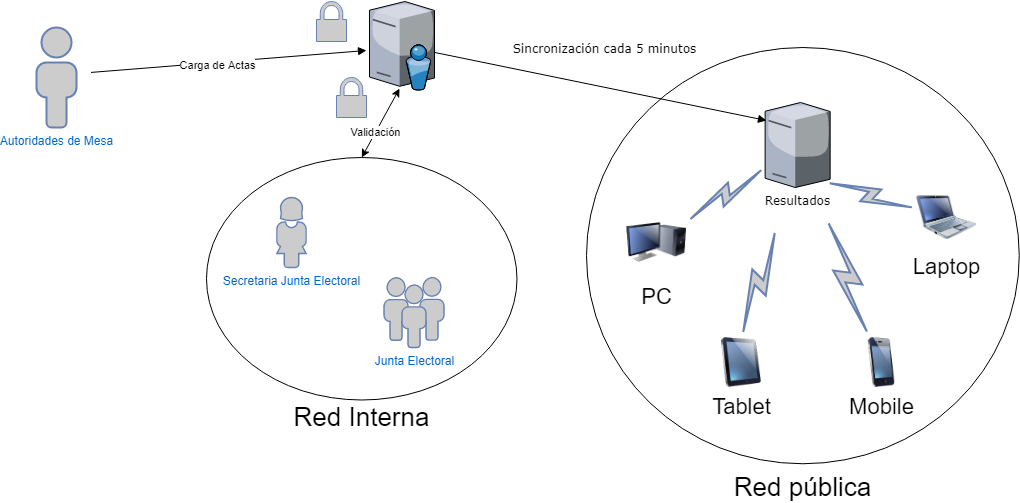
\includegraphics[width=\textwidth]{img/arquitectura.png}
  \caption{Arquitectura}
  \label{graf:arquitectura}
\end{figure}

Gukena se implementó sobre una arquitectura dividida en tres módulos (imagen \ref{graf:arquitectura}) que se relacionan con los diferentes roles que interaccionan con el sistema.
\begin{itemize}
\item Módulo Resultados: muestra los resultados en un servidor web público, para que la comunidad universitaria pueda conocer los resultados a medida que se van cargando los datos.
\item Módulo Autoridad de Mesa: desde cualquier dispositivo con conexión a Internet las Autoridades de Mesa acceden con su usuario y clave para cargar los datos del acta desde el lugar de votación.
\item Módulo Junta Electoral: los integrantes de la junta electoral y la Secretaria realizan un doble chequeo de las actas cargadas por las Autoridades de Mesa en una red interna.
\end{itemize}

La propiedad de usabilidad es importante para que un sistema sea fácil de aprender y de utilizar. Cada uno de estos módulos implican actividades disjuntas dentro del sistema, por lo tanto, para cada rol se le dispuso una interacción distinta con el sistema. \newline
El público en general tiene la necesidad de ver los resultados parciales durante el proceso de escrutinio, para cumplir este objetivo se accede a Gukena a través del sitio público de resultados \footnote{Sitio resultados: \url{https://resultados.uncoma.edu.ar}}.
Esta página es accesible desde cualquier navegador, contiene un historial de elecciones, categorías de búsqueda de información, gráficos y descripciones explicativas sobre los datos visualizados. Por otro lado, el rol de autoridad de mesa tiene la necesidad de transmitir la información del resultado de su escritinio, por este motivo acceden a sitio \footnote{Sitio Autoridades de Mesa y Junta Electoral: \url{https://gukena.fi.uncoma.edu.ar/}},
donde se loguean con la información recibida previamente y acceden a una única pantalla con un formulario correspondiente a la mesa escrutada. Por último tenemos al módulo de Junta Electoral quienes necesitan validar y/o corregir la información cargada en el sistema. Acceden al mismo link que una autoridad de mesa con la diferencia que al validar múltiples mesas, el sistema le dispone un listado de todas las mesas, con filtros y categorías para facilitar su búsqueda. Además, cada mesa se encuentra etiquetada con información sobre su estado, es decir, si ya fue cargada por la autoridad de mesa correspondiente o en la espera de su carga. Por cada mesa se le despliega la misma pantalla que se dispone a una autoridad de mesa para que pueda hacer las correcciones necesarias con una acción de validar esta información. Cabe destacar que una autoridad de mesa solo tiene disponible el formulario de carga hasta que envia la información cargada, a partir de ese momento solo puede visualizar el formulario pero no volver a editarlo.\newline

%\agregar{citaa LAMP - HECHO}
Por otro lado, a nivel técnico Gukena se desarrolló sobre una infraestructura web LAPP como variación a la arquitectura LAMP. Las siglas LAMP corresponde al paquete open source  \cite{chaparro2006lamp} que contiene: 
\begin{itemize}
    \item Linux: Sistema Operativo basado en software libre.
    \item Apache: Servidor web.
    \item MySQL: Servidor de base de datos relacionales open source.
    \item PHP: Lenguaje de programación open source embebido en páginas HTML, ejecutado en el servidor. Compatible con distintos sistemas operativos y bases de datos.
\end{itemize} Gukena se implementó sobre un sistema base Linux, servidor web Apache, el lenguaje de programación PHP y como variación utilizó el sistema gestor de base de datos PostgreSQL. 


\subsection{Modelo de datos}
 %\cambiar{hablaría de entidades en vez de clases}

La semántica de este problema se representó sobre una base de datos relacional utilizando herramientas de software libre. Se utilizó el Gestor de Base de Datos PostgreSQL sobre un sistema operativo Linux. El modelo de datos representa los conceptos más importantes en un dominio. Conociendo el proceso de elección en la Universidad Nacional del Comahue se observan las entidades más importantes que son: unidad electoral, mesas, claustros, actas y las listas oficializadas para cada cargo. En base a estos conceptos principales tenemos los votos que recibe cada lista postulada que se agrupan por las sedes que conforman cada Unidad Electoral. Además para mantener el histórico de elecciones se tiene la entidad Acto Electoral manteniendo las fechas de cada elección realizada.\newline
Conociendo el modelo de datos, al momento de una nueva elección es necesario realizar una precarga de datos sobre:
\begin{itemize}
    \item Acto electoral con fecha de la nueva elección, asociando los claustros que votarán y las unidades electorales y sedes participantes
    \item Datos de las mesas: número de mesa, cantidad de empadronados en cada mesa, claustro al que pertenece.
    \item Listas oficializadas para cada claustro y el cargo al que se postula
    \item Usuarios habilitados a ingresar al sistema
\end{itemize}
%\cambiar{Diagrama del modelo de datos que representa las relaciones de la tablas en la Bases de Datos PostgreSQL - HECHO}
\begin{figure}[h!]
  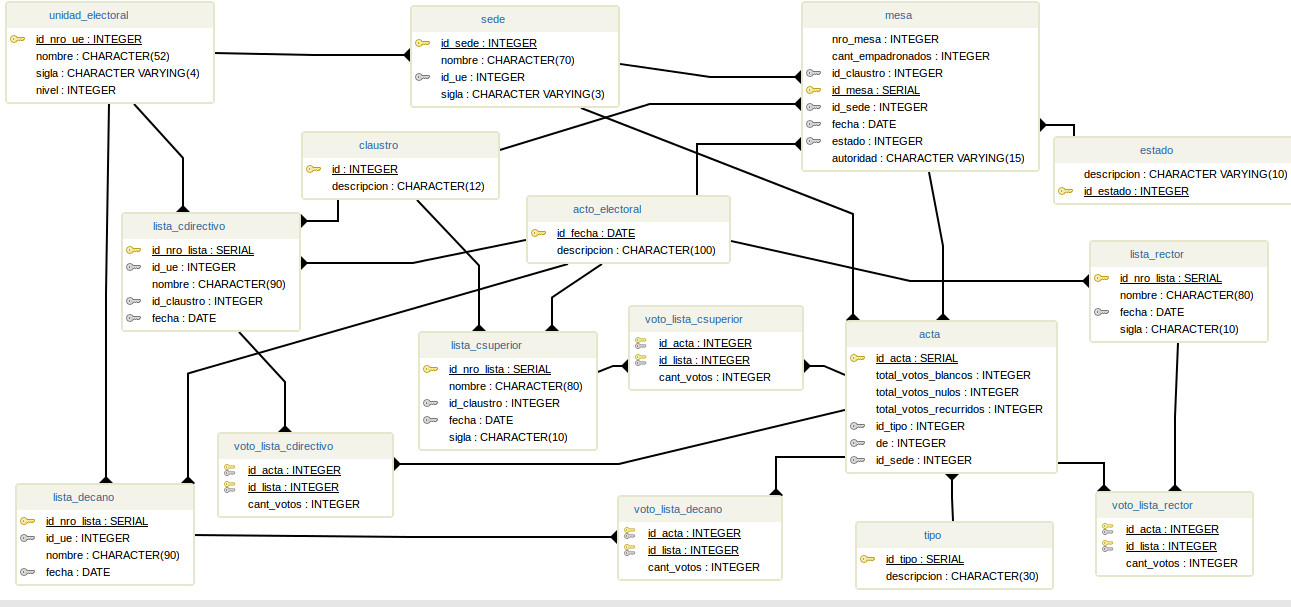
\includegraphics[width=\textwidth]{img/gu_kena_diagramaBD.jpg}
  \caption{Relación entre las tablas almacenadas en la Base de Datos Gukena}
  \label{graf:diagramaBD}
\end{figure}

Este modelo de datos representado en la Figura \ref{graf:diagramaBD} es el almacenamiento principal del sistema, es decir, la carga de datos por parte de las autoridades de mesa y Junta Electoral y, el procesamiento de los resultados impacta sobre esta fuente de datos. 

\subsection{Interoperabilidad externa}
%\agregar{Agregar que se trata de una API REST.  Describir y citar que significa API REST. Poner un link real a modo de ejemplo - REVISAR}
Un programa ejecutado del lado cliente se comunica con los servicios web a través de APIs (Application Programming Interfaces). Las APIs exponen un conjunto de datos y funciones para facilitar la interacción entre programas y así poder intercambiar información. El estilo de arquitectura REST es aplicado comúnmente en el diseño de APIs de servicios web modernos. Por lo tanto, una API web implementado con esta arquitectura es un API REST. \cite{masse2011rest}

Gukena expone este conjunto de datos a través de archivos en formato JSON con una arquitectura propia que permite su fácil consulta desde programas cliente. Estos archivos son actualizados durante el escrutinio cada 5 minutos y son el resultado de procesar los datos existentes en la base de datos SQL. Estos archivos son consumidos por la página de Gukena pública, sin embargo, pueden ser consultados por cualquier sistema o persona que los quiera acceder. A continuación se describe brevemente la estructura y notación utilizada para un acceso externo a Gukena.
La estructura de estos archivos está formada por:
\begin{itemize}
    \item data (lista, sigla , total de votos, sede)
    \begin{itemize}
        \item lista (String)
        \item sigla (String)
        \item total de votos (int)
        \item sede (int)
    \end{itemize}
    \item columns (field , title)
    \begin{itemize}
        \item field (String)
        \item title (String)
    \end{itemize}
    \item titulo (String)
    \item labels (String)
    \item total (int)
    \item fecha (datetime)
    \item enviados y confirmadas (String)
    \item titulo\_grafico (String)
\end{itemize}
Para reconocer que archivo se debe consumir para obtener los datos deseados,  se aplicó una notación conformada por \textbf{nombreCargo} + \textbf{siglaUnidadElectoral} + \textbf{nombreClaustro} + \textbf{".json"} en el nombre de cada archivo. En la tabla \ref{tab:formatoJSON} se representa este formato.

\begin{table}[htbp]
\begin{center}
\begin{tabular}{|l|l|l|}
\hline
Categoria\_ & Unidad\_Electoral & \_ Claustro.json\\
\hline \hline 
R(Rector) & Todo(Universidad) & T(Total)\\ \hline
D(Decano) & ASMA & D(Docentes)\\ \hline
CD(Consejo Directivo) & AUZA & E(Estudiantes)\\ \hline
CS(Consejo Superior) & CRUB & G(Graduados)\\ \hline
-& CUZA & N(No Docentes) \\ \hline
-& ESCM &- \\ \hline
-& FACA &- \\ \hline
-& FACE &- \\ \hline
-& FADE &- \\ \hline
-& FACA &- \\ \hline
-& FAEA &- \\ \hline
-& FAHU &- \\ \hline
-& FAIF &- \\ \hline
-& FAIN &- \\ \hline
-& FALE &- \\ \hline
-& FAME &- \\ \hline
-& FATA &- \\ \hline
-& FATU &- \\ \hline
\end{tabular}
\end{center}
\caption{Nombre de archivos JSON}
\label{tab:formatoJSON}
\end{table}

\subsection{Seguridad}
Las vulnerabilidades de un software afectan a la seguridad de un sistema, estos pueden ser debilidades funcionales o lógicos.
Descubrir estas vulnerabilidades es importante para proteger la información. \cite{definicionVulnerabilidad}.
%\agregar{cita OWASP y tablita resumen de posibles ataques y formas de mitigarlos - HECHO}

Se ha contemplado y evaluado la Seguridad en cada fase  del diseño e implementación del sistema.  La principal amenaza es que se vulnere el enlace con los usuarios que cargan y verifican los datos.  Por esta razón, los tres módulos están publicados en un servidor web Apache a través del protocolo HTTPS para asegurar el enlace. Además, la verificación de la Junta Electoral y la confirmación de la Secretaría se realizan dentro de una red interna. \newline
%\cambiar{Así mismo,} 
Así mismo, no existe un enlace directo entre los datos del escrutinio cargado al sistema y los datos visualizados por el
público. Los datos procesados son depositados en archivos con formato JSON los cuales son actualizados continuamente cada 5 minutos por un script interno y, estos archivos son levantados por la página web para su correcta visualización. \newline
Existe una fundación sin fines de lucro OWASP (Open Web Application Security Project) \footnote{URL: https://owasp.org/} cuyo objetivo es mejorar la seguridad del software. OWASP Top 10 es un documento estándar de conscientización para desarrolladores sobre la seguridad en aplicaciones web. Este documento contiene los 10 riesgos más críticos en seguridad, el ranking obtenido en el 2020 se representa en la tabla \ref{tab:top10}.

\begin{table}
  \begin{tabular}{p{0.35\textwidth}p{0.65\textwidth}}
    \toprule
Riesgo & Prevención\\
    \midrule
    1.Inyección & \tabitem Parametrizar las consultas \\
    & \tabitem Validar los datos ingresados  \\
    & \tabitem Escapar caracteres especiales  \\
    \hline
    2.Autenticación rota & \tabitem Usar buenas librerias de autenticación\\
    & \tabitem Forzar el uso de contraseñas fuertes \\
    & \tabitem Detectar y prevenir ataques de fuerza bruta \\
    \hline
    3.Datos sensibles expuestos & \tabitem No guardar datos que no se necesiten\\
    & \tabitem Usar un encriptado fuerte \\
    \hline
    4.XML Entidades Externas (XXE) & \tabitem Evitar XML\\
    & \tabitem Usar librerías modernas con una buena configuración \\
    & \tabitem Validar XML \\
    \hline
    5.Control de acceso rota & \tabitem Usar códigos o librerías probadas\\
    & \tabitem Por defecto denegar el acceso \\
    & \tabitem Guardar fallas y alertar \\
    & \tabitem Acceso limitado en accesos a recursos \\
    \hline
    6.Mala configuración de seguridad & \tabitem Deshabilitar servicios no usados\\
    & \tabitem Usar herramientas para revisar configuraciones \\
    \hline
    7.Cross-site Scripting (XSS) & \tabitem Codificar todos los datos recibidos del usuario\\
    & \tabitem Usar una codificación apropiada al contexto \\
    & \tabitem Usar frameworks que genere HTML seguro \\
    & \tabitem Usar política de seguridad de contenido \\
    \hline
    8.Deserealización insegura & \tabitem Evitar serializar y deserealizar objetos\\
    & \tabitem Usar firmas para detectar manipulaciones\\
    & \tabitem Configurar librerias seguras \\
    & \tabitem Limites de accesos a recursos \\
    \hline
    9.Utilización de componentes con vulnerabilidades conocidas 
    & \tabitem Reducir dependencias\\
    & \tabitem Parches admnistradas \\
    & \tabitem Escanear componentes vencidos\\
    & \tabitem Presupuestar por el mant. continuo de todos los proyectos de software \\
    \hline
    10.Logging y monitoreo insuficientes \\
    \bottomrule
  \end{tabular}
  \caption{OWASP Top 10}
\label{tab:top10}
\end{table}


Como se puede ver existen distintos tipos de ataques a los datos de un sistema con el fin de obtener información, manipularlos o destruirlos. El término Inyección por SQL consiste en la inserción de código SQL por medio de los datos de entrada desde el lado de cliente hacia el servidor. Es decir, por medio de la inserción de este código el atacante puede modificar las consultas originales que debe realizar la aplicación y ejecutar otras totalmente distintas con la intención de acceder a la herramienta, obtener información de alguna de las tablas o borrar los datos almacenados, entre otras muchas cosas. Al conocer este término se puede ver que debido a que la página utiliza archivos para alimentarse y no realiza consultas SQL directas a la base de datos, este tipo de ataque no es posible. Como mayor daño podría llegar a ser manipular o destruir estos archivos, que luego son reemplazados nuevamente de manera automática por el sistema con los datos reales y correctos. \newline
Otro de los ataques que se nombraron es el acceso no autorizado al sistema con el objetivo de manipular los datos cargados del escrutinio en una mesa en particular, o un conjunto de ellas. Los usuarios con los roles de Autoridad de mesa, Junta Electoral y Secretaría tienen login con nombre de usuario y clave para ingresar al sistema. Esta información es enviada de manera impresa dentro de un sobre cerrado con la instrucción de que la persona encargada del cierre de la mesa de votación lo abra para ingresar al sistema. Además se registra cada acción de inserción y modificación que se realiza en los formularios del sistema en un log general para cubrir el riesgo 10 nombrado en el ranking. \newline

\subsection{Proceso de la Elección}

El procedimiendo electoral en la Universidad Nacional del Comahue se rige a través de la Ordenanza Nº1386/13, del Consejo Superior de la Universidad Nacional del Comahue \cite{ordenanzaUncoma}. Luego de varias elecciones exitosas dentro del ámbito, se establece una metodología a utilizar para computar los resultados de actos electorales realizados en el ámbito de la Universidad Nacional del Comahue, utilizando un sistema de escrutinio descentralizado. \newline
El proceso electoral utilizando Gukena se compone de los siguientes pasos:
%\agregar{Paso 1: Carta marina. Carga de listas ...}
\begin{itemize}

\item Paso 1: Carta marina. Carga de listas y mesas. Se carga la información de las listas de candidatos oficializadas y las mesas electorales con su respectiva cantidad de empadronados.
\item Paso 2: Se validan los datos cargados en el Sistema. Se corrobora que la información cargada en la Base de Datos del Sistema gukena es la misma que la que fue oficializada por la Junta Electoral.
\item Paso 3: Sobres con usuario. Se arma un sobre para cada mesa que contenga la información del Usuario y la Contraseña para poder acceder al sistema. Ejemplo en la imagen \ref{graf:ejemploSobre}

\begin{figure}[h!]
    \begin{center}
        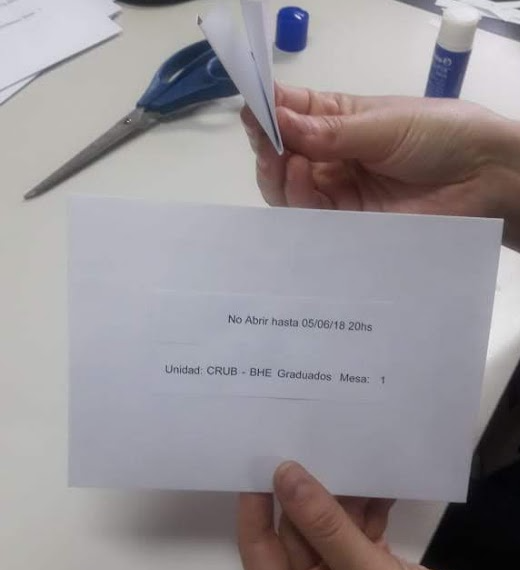
\includegraphics[scale=0.5]{img/jKz6EB2F9Z.png}
    \end{center}
  \caption{Ejemplo Sobre enviado dentro de la urna de la mesa nº1}
  \label{graf:ejemploSobre}
\end{figure}

\item Paso 4: Envío de material. Se envía a cada dependencia el material necesario para poder llevar a cabo los comicios, incluyendo un breve instructivo de carga para la Autoridad de Mesa y el sobre cerrado nombrado en el paso anterior (que sólo debe ser abierto al momento de cargar el acta en el sistema).
\item Paso 5: El Acto Electoral se lleva a cabo en las fechas fijadas por el cronograma electoral y cumpliendo con lo especificado en la Ordenanza Nº 1386/13.
\item Paso 6: Escrutinio Provisorio de la Mesa. 
Una vez que haya finalizado el Acto Electoral, las Autoridades de Mesa realizan el escrutinio provisorio de los votos obtenidos en su mesa, para luego completar por duplicado el acta en papel con la información obtenida del recuento. Ejemplo de un acta cargada en la imagen \ref{graf:ejemploActa}.

\begin{figure}[h!]
    \begin{center}
        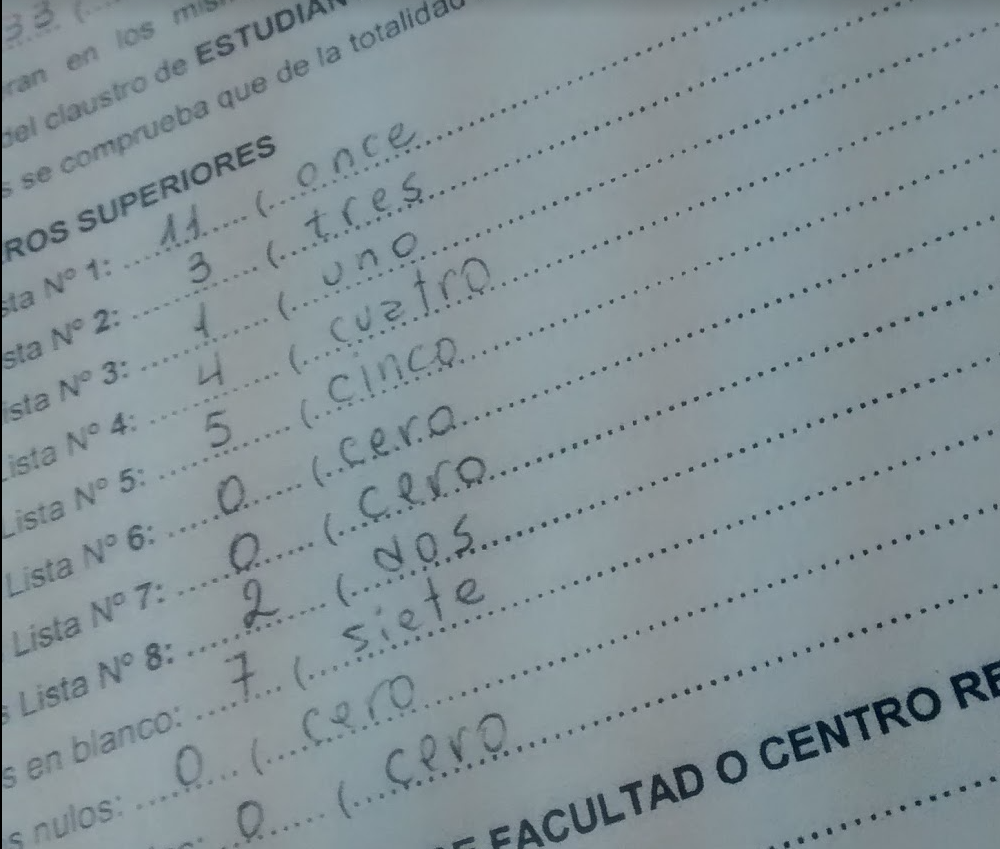
\includegraphics[scale=0.25]{img/f4P4qmrKXY.png}
    \end{center}
  \caption{Ejemplo Acta en papel completada por una Autoridad de Mesa}
  \label{graf:ejemploActa}
\end{figure}

\item Paso 7: Finalizado el Acto Electoral, se habilita el Sistema Gukena para que pueda ingresar cada Autoridad de mesa.
\item Paso 8: Carga y envío de datos en Gukena. Una vez que haya completado el acta papel, la Autoridad de Mesa carga la información de ésta en el Sistema Gukena. Para esto deben ingresar al mismo utilizando el usuario y contraseña contenidos en el sobre. Ejemplo de la pantalla del login en la imagen \ref{graf:ejemploLogin}.
Cuando los datos del acta son confirmados o enviados por la Autoridad de Mesa, estos datos ya no pueden ser editados por este usuario.

\begin{figure}[h!]
    \begin{center}
        
\includegraphics[scale=0.5]{img/ZJ3mtjmmdZ.png}
    \end{center}
  \caption{Pantalla de login para el módulo Autoridad de Mesa y Junta Electoral}
  \label{graf:ejemploLogin}
\end{figure}

\item Paso 10: La Autoridad de Mesa deposita un ejemplar del acta dentro de la urna antes de cerrarla y otro ejemplar es enviado a la Junta Electoral, enviada por los medios disponibles por la Autoridad de Mesa, por ejemplo fax, email, entre otros. 
\item Paso 11: Primera Validación de datos. La Junta Electoral confirma en el sistema que los datos cargados, por las autoridades de mesa, coinciden con las actas papel recibidas, permitiendo corregir cualquier error ocurrido durante el proceso de carga. Para aquellas actas que, por algún inconveniente, no fueran cargadas por la Autoridad de Mesa, como se especifica en el paso anterior, deben ser cargadas por algún miembro de la Junta Electoral.
\item Paso 12: Segunda Validación de los datos. La Secretaria de la Junta Electoral realiza una segunda validación de las actas ya confirmadas por la Junta, en el caso de encontrar diferencias devuelve el acta a la Junta Electoral para su corrección. Si no hay diferencias, entonces dicha acta queda confirmada en el sistema. Una vez que el acta es confirmada ya no puede ser modificada por ningún miembro de la Junta Electoral.

\end{itemize}


\section{Desarrollo}
Gukena ha sido construido por el Grupo de Desarrollo Euclides \footnote{Euclides: http://euclides.uncoma.edu.ar/?q=somos} que está integrado por un conjunto de no docentes, estudiantes avanzados y docentes de la Facultad de Informática en la Universidad Nacional del Comahue y funciona bajo la dirección de la Subsecretaría de Tecnologías de la Información de la misma Universidad. El sistema se desarrolló durante los meses de abril a junio a partir del 2015 y los años siguientes, integrándose mejoras evolutivas en cada año.

Para el desarrollo del sistema se utiliza el modelo de ciclo de vida iterativo e incremental, basado en la metodología Scrum, para promover un proceso de construcción ágil y una comunicación fluida con el cliente y, conseguir los beneficios del sistema de forma incremental. En 2015 una primera versión se utilizó para validar las planillas usadas hasta el momento, en 2016 y 2017 se empleó el sistema de forma completa.  En 2018 fue la primera vez que se utilizó en una elección completa considerando los cuatro claustros y los cargos de Rector, Decano, Consejeros Directivos y Superiores. Este año se aplicaron mejoras sobre las pantallas accesibles por el público en general que permiten ver los resultados parciales en tiempo real, junto a un histórico de elecciones. Esta mejora fue bien aceptada por la comunidad universitaria permitiendo a los medios de comunicación y público en general tener un acceso rápido a los resultados.

En la construcción, diseño e implementación de Gukena se utilizan solamente herramientas de software libre. Se usa el ambiente desarrollo web SIU Toba \footnote{SIU Toba: https://www.siu.edu.ar/siu-toba/}, que es desarrollado por el consorcio SIU para soluciones del Sistema Universitario Nacional. Esta herramienta  permite crear sistemas transaccionales en forma rápida, utilizando tecnología web open-source y su objetivo es agilizar el proceso de construcción y el mantenimiento de los mismos y, de esta manera se permite al equipo de desarrollo enfocar su actividad en la lógica del dominio.  El ambiente integra el lenguaje de programación PHP, servidor web Apache, sistema operativo Linux y bases de datos PostgreSQL, entre otros.

Se trabaja utilizando con la filosofía del desarrollo de código abierto, para contribuir a mejorar el mantenimiento del sistema. Los fuentes son de licencia libre y acceso público, se encuentran disponibles en un repositorio libre
\footnote{Github: \url{https://github.com/svs07uni/gu_kena}} 
con la intención  de que la comunidad de desarrolladores, investigadores, y comunidad de la Universidad puedan acceder al software y analizarlo.
%\agregar{reformular descripción MVC toba con fragmentos de código y gráfico}
El ambiente de desarrollo web SIU Toba está basado en el patrón arquitectónico MVC (Model, View, Controller), el cual separa los datos de una aplicación, la interfaz de usuario y la lógica de control en tres componentes distintos.
Este patrón permite la separación de conceptos, características que buscan facilitar la tarea de desarrollo de aplicaciones y su posterior mantenimiento. Por lo tanto, este tipo de arquitectura permitió dividir tareas de desarrollo dentro del grupo Euclides y permitió facilitar su evolución por cada año de experiencia. \newline
De manera genérica los componentes de MVC se pueden describir como:
\begin{itemize}
    \item Model (Modelo): Es la representación de la información con la cual el sistema opera y gestiona todos los accesos a dicha información. En este contexto, el Modelo permite guardar y consultar los datos del escrutinio final por cada mesa. Además este componente se encargó de aplicarle las fórmulas necesarias para conseguir el resultado provisorio y/o final de la distribución de escaños. Otra información importante que gestionó fue el log de actualizaciones sobre estos datos, esto permite satisfacer las propiedades de auditabilidad, ya que se registran las actualizaciones por parte de las autoridades de mesa y personal de la Junta Electoral autorizada.
    \item View (Vista): Presenta el Modelo de una manera adecuada para interactuar, es decir, la interfaz de usuario. Se encarga de la representación visual de los datos que gestiona el Modelo. Gukena dispuso una vista por cada módulo de interacción. De manera tal que una autoridad de mesa solo accede a un formulario de carga, una persona autorizada de la Junta Electoral accede a un listado de mesas a validar, y por último una vista más gráfica para el módulo de Resultados. Este componente tiene la responsabilidad de satisfacer las propiedades de usabilidad del sistema.
    \item Controller (Controlador): Responde a eventos e invoca peticiones al Modelo, se encarga de controlar las acciones del usuario y de solicitar los datos al Modelo para comunicarselos a la vista. En Gukena, el Controlador suministró los datos mediante dos vias, una de ellas es la comunicación directa entre Vista y Modelo para los módulos de Autoridad de Mesa y Junta Electoral, sin embargo, para el módulo de Resultados el controlador 'empaquetaba' los datos y los depositaba en archivos JSON, los cuales eran el origen de datos para este módulo.
\end{itemize}
*En la Figura \ref{graf:mvcArquitectura} se puede ver las interacciones entre estos componentes para lograr que el Usuario acceda a los Datos del sistema. Uuna de las ventajas de esta arquitectura MVC es que permite separar los componentes de una aplicación dependiendo de la responsabilidad que tienen. Esto respeta el principio de la responsabilidad única.

\begin{figure}[h!]
    \begin{center}
        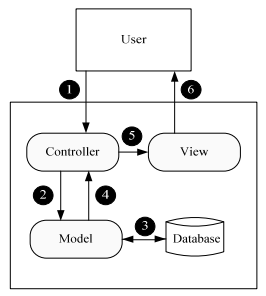
\includegraphics[scale=0.5]{img/mvc_arq.png}
    \end{center}
  \caption{Arquitectura del Framework}
  \label{graf:mvcArquitectura}
\end{figure}

SIU Toba respeta notaciones para referir a cada uno de estos componentes, por ejemplo en la imagen \ref{graf:ejemploPantalla} se puede ver una parte del código de configuración sobre el controlador asociado a la mesa. Al tener la palabra ´´conf'' refiere a la configuración y la palabra ´´pant'' se asocia a la pantalla denominada ´´edicion''. De igual modo, se puede observar como se accede al Modelo dentro de este framework con la siguiente linea
\begin{lstlisting}
$this->dep('datos')->tabla('nombreTabla')}
\end{lstlisting}
Esta arquitectura ayuda a su mantenimiento ya que el código queda más prolijo y claro.

\begin{figure}[h!]
    \begin{center}
        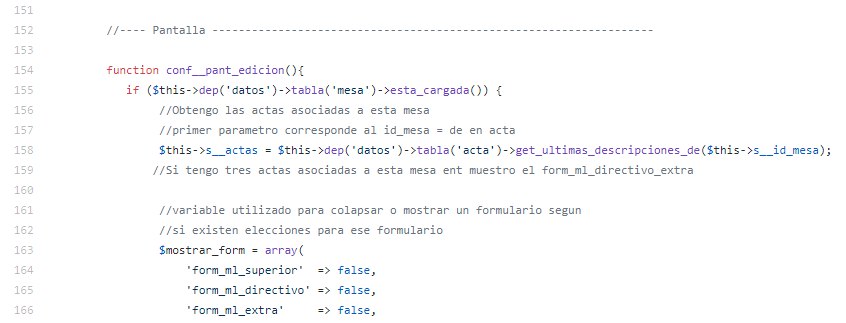
\includegraphics[scale=0.5]{img/ejemplo_pantalla.png}
    \end{center}
  \caption{CI Mesa - Carga de pantalla de Edición de una mesa}
  \label{graf:ejemploPantalla}
\end{figure}

\section{Testing}
El Testing de un software es cualquier actividad cuyo objetivo es evaluar un atributo o la capacidad de un programa o sistema y determina si logró encontrar los resultados esperados \cite{pan1999software}. Esto no significa que únicamente se utiliza para debuggear un software, el propósito del Testing es asegurar la calidad, verificación y validación, o estimación de confiabilidad. Esta actividad contiene métodos y técnicas destinadas a múltiples propósitos durante las fases dentro de un desarrollo de software. Testing se puede dividir como: testing de correctitud, testing en performance, testing en confiabilidad y testing de seguridad. Un tester puede abocarse a verificar la correctitud de un sistema o software sin conocer internamente su funcionamiento, conocido como testing de caja negra (black-box testing) o por el contrario, planificar los casos de test de acuerdo a los detalles de implementación del software (testing de caja blanca o white-box testing). \newline
Para los casos de test en Gukena participó el equipo que lo desarrollo y usuarios externos a este, como docentes de la Facultad de Informática. Los casos de test involucraron:
\begin{itemize}
    \item Carga de datos erróneos en los formularios de carga del rol Autoridad de mesa, por ejemplo valores negativos en los formularios.
    \item Verificar validaciones integradas en los formularios que conforman la pantalla de carga del rol Autoridad de mesa, por ejemplo las validaciones contra la cantidad de empadronados, validaciones en la cantidad de votantes cargadas en cada formulario.
    \item Verificar cambios de estado de una mesa desde el guardado hasta la validación final por el rol Junta electoral.
    \item Verificar los datos procesados por una cantidad reducida de mesas cargadas contra el resultado final generado por el sistema.
    \item Accesos no autorizados por usuarios no permitidos.
    \item Testing de sobrecarga en consultas paralelas con una cantidad reducida de dispositivos en un mismo instante.
\end{itemize}